\section{Introduction}
\label{sec:introduction}

% state the learning objective 
The objective of this laboratory assignment is to study a circuit with 4 meshes, containing a total of 7 resistors (from $R_1$ to $R_7$), 2 current sources ($I_d$ and $I_b$), one of them, $I_b$, linearly voltage-controlled (VCCS), and 2 voltage sources ($V_a$ and $V_c$), one of them, $V_c$, linearly current-controled (CCVS). The circuit can be seen in Figure~\ref{fig:rc}.

In Section~\ref{sec:analysis}, a theoretical analysis of the circuit is
presented. In Section~\ref{sec:simulation}, the circuit is analysed by
simulation, and the results are compared to the theoretical results obtained in
Section~\ref{sec:analysis}. The conclusions of this study are outlined in
Section~\ref{sec:conclusion}.

\begin{figure}[h] \centering
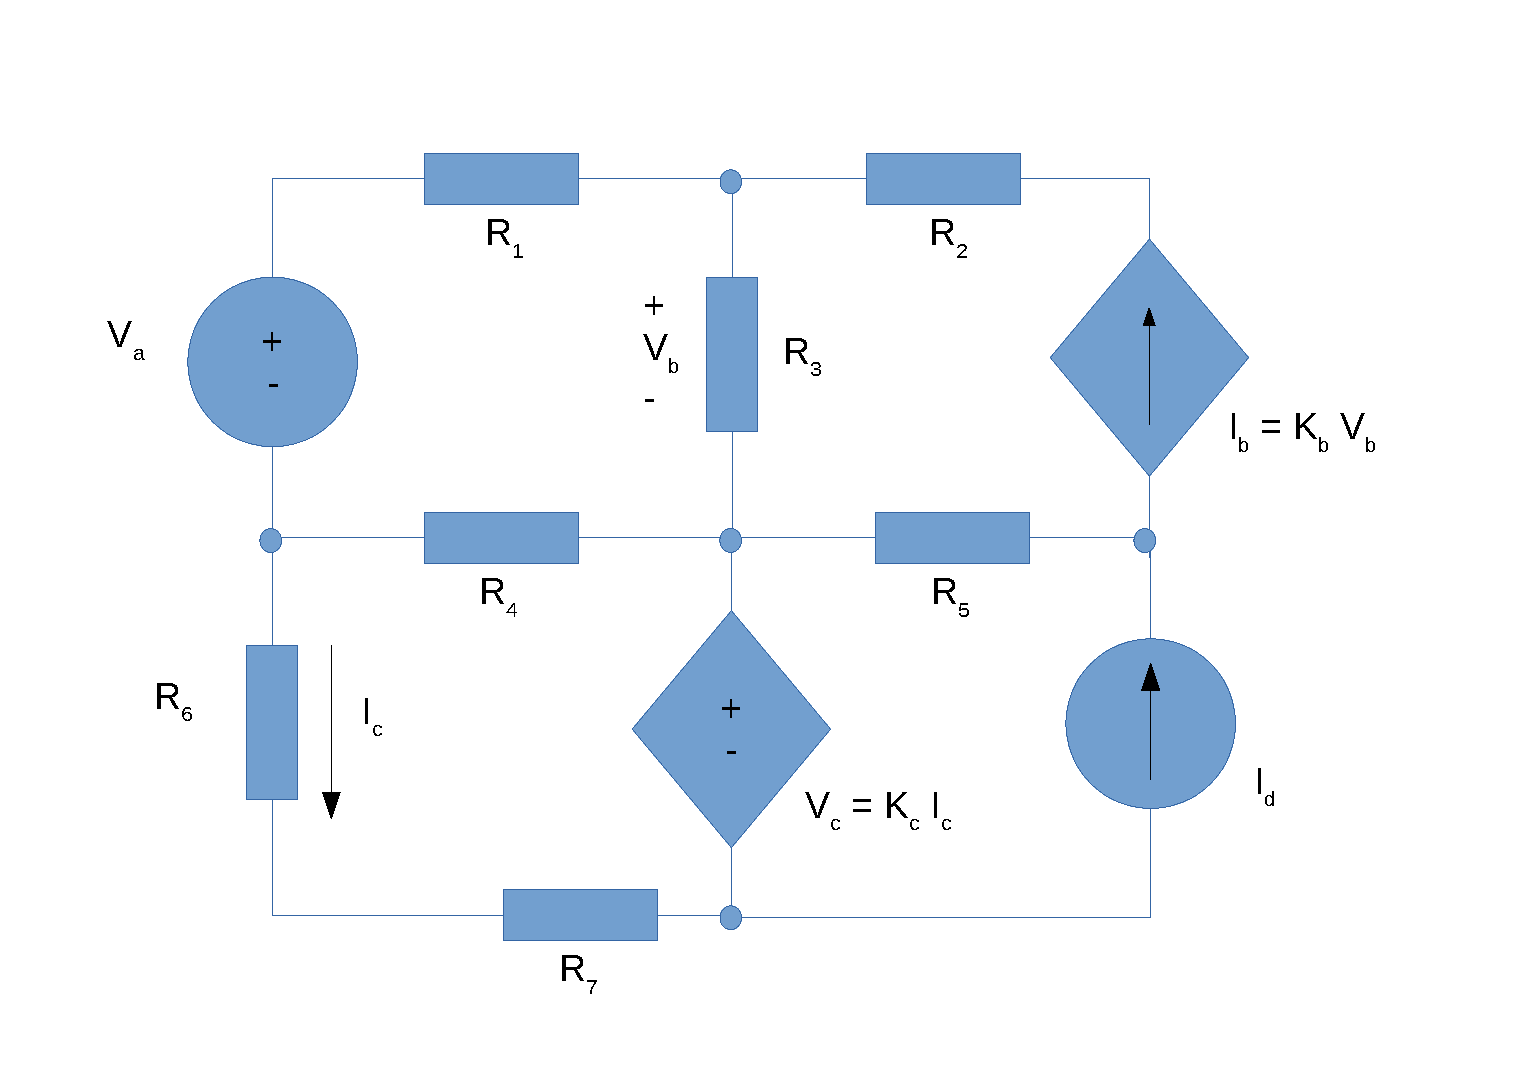
\includegraphics[width=0.4\linewidth]{circuit_intro.pdf}
\caption{Circuit of of Laboratory no 1.}
\end{figure}

